\documentclass[conference]{IEEEtran}
\usepackage{blindtext, graphicx}
\usepackage{amsmath}
\usepackage{listings}


\ifCLASSINFOpdf
\else
\fi


% correct bad hyphenation here
\hyphenation{op-tical net-works semi-conduc-tor}


\begin{document}

\title{Chimera: Agnostic Language Component Based Framework using NodeJS and CLI}

\author{\IEEEauthorblockN{Go Frendi Gunawan}
\IEEEauthorblockA{STIKI Malang\\
Malang, Indonesia\\
Email: frendi@stiki.ac.id}
\and
\IEEEauthorblockN{Mukhlis Amien}
\IEEEauthorblockA{STIKI Malang\\
Malang, Indonesia\\
Email: amien@stiki.ac.id}
\and
\IEEEauthorblockN{Jozua Ferjanus Palandi}
\IEEEauthorblockA{STIKI Malang\\
Malang, Indonesia\\
Email: jozuafp@stiki.ac.id}}

% make the title area
\maketitle


\begin{abstract}
%\boldmath
    Component Based Software Engineering (CBSE) is a popular topic in Software Engineering. The main advantage of CBSE is separation of components. A single component will only focus on a single task or related collection of tasks. Allowing software developer to reuse the component for other use-cases. By using this approach, software developer doesn't need to deal with spaghetti code. Several approaches has been developed in order to achieve ideal CBSE. The earliest implementation was unix pipe and redirect, while the newer approach including CORBA, XML-RPC, and REST. Our framework, Chimera, was built on top of Node JS. Chimera allows developer to build pipe flow in a chain (a YAML formatted file) as well as defining global variables. Compared to unix named and unnamed pipe, this format is easier and more flexible. On the other hand, unlike XML-RPC, REST, and CORBA, chimera doesn't enforce users to use http protocol.
\end{abstract}

% Note that keywords are not normally used for peerreview papers.
\begin{IEEEkeywords}
Chimera, Language Agnostic, Component-Based Software Engineering, Node JS, CLI.
\end{IEEEkeywords}

\IEEEpeerreviewmaketitle



\section{Introduction}
\blindtext
\cite{def:feilhauer}

\iffalse
\begin{equation}
p(C_{k},x_{1},\dots ,x_{n})\,
\end{equation}

\begin{equation}
E(v,h) = - b'v - c'h - h'Wv
\label{eq:rbm1}
\end{equation}

\begin{figure}
	\centering
	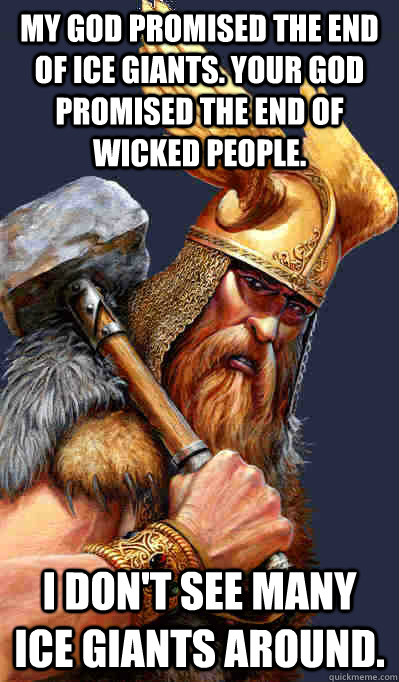
\includegraphics[width=0.3\textwidth]
		{ice.jpg}
	\caption{Ice Giant}
	\label{fig:bon1}
\end{figure}

\begin{lstlisting}[caption=Contoh listing, label=mult1, basicstyle=\small, language=java]
public static void main(String[] args) {
	System.out.println("Hello World");
}

\end{lstlisting}

Fungsi energi $E(v,h)$ pada RBM didefinisikan sebagai persamaan \ref{eq:rbm1}.
\fi




\subsection{Subsection Heading Here}
\blindtext


\section{Conclusion}
\blindtext


\appendices
\section{Proof of the First Zonklar Equation}
\blindtext

% use section* for acknowledgement
\section*{Acknowledgment}
The authors would like to thank...

% Can use something like this to put references on a page
% by themselves when using endfloat and the captionsoff option.
\ifCLASSOPTIONcaptionsoff
  \newpage
\fi

\begin{thebibliography}{1}

\bibitem{def:feilhauer}
Feilhauer, T. and Sobokta, M., DEF - A Programming Language Agnostic Framework and Execution Environment for The Parallel Execution of Library Routines, Journal of Cloud Computing: Advances, Systems and Applications (2016) 5:20

\bibitem{parallel:conway}
Conway, T., Parallel Processing on the Cheap: Using Unix Pipes to Run SAS Programs in Parallel, Sugi 28, Seattle, Washington, March 30 - April 2, 2003 

\bibitem{mass:mcilroy}
Mcilroy, M. D., Mass Produced Software Components, Report on a conference sponsored by the NATO SCIENCE COMMITTEE, Garmisch, Germany, 7th to 11th October 1968



\end{thebibliography}

\begin{IEEEbiography}[{\includegraphics[width=1in,height=1.25in,clip,keepaspectratio]{picture}}]{John Doe}
\blindtext
\end{IEEEbiography}



% that's all folks
\end{document}

